\documentclass[english,handout]{mlutalk}

\title{Stance Classification for Key-Point Analysis}
% \title{%
%   Modern Talking: Key-Point Analysis \\
%   using Modern Natural Language Processing
% }
\subtitle{Natural Language Processing, Summer Semester 2021}
\author{Max Henze \and Hanh Luu \and Jan Heinrich Reimer}
\institute{Martin Luther University Halle-Wittenberg}
\date{April 20, 2021}
\titlegraphic{
\includegraphics[width=3cm]{figures/mlu-halle}}

\addbibresource{../literature/literature.bib}

\usepackage{tikz}
\usetikzlibrary{positioning}
\usepackage{listings}
\usepackage{xspace}
\usepackage{biblatex}
\usepackage{tabularx}
\usepackage{booktabs}
\usepackage{graphics,graphicx}

\newcommand{\Bert}{\textsc{Bert}\xspace}
\newcommand{\ArgKP}{\mbox{ArgKP}\xspace}
\newcommand{\ArgQ}{\mbox{IBM-ArgQ-Rank-30kArgs}\xspace}
\newcommand{\BiLSTM}{\mbox{BiLSTM}\xspace}
\newcommand{\BertBase}{\textsc{Bert}-Base\xspace}
\newcommand{\BertLarge}{\textsc{Bert}-Large\xspace}
\newcommand{\TF}{\mbox{TF}\xspace}
\newcommand{\TFIDF}{\mbox{TF/IDF}\xspace}

\tikzset{%
    every neuron/.style={
      circle,
      draw,
      minimum size=1cm
    },
    neuron missing/.style={
      draw=none, 
      scale=4,
      text height=0.333cm,
      execute at begin node=\color{black}$\vdots$
    },
    layer/.style= {
      rectangle,
      draw,
      minimum size = 1cm
    }
  }

\begin{document}

\titleframe

\begin{frame}
  \frametitle{Brainstorming}

  \begin{itemize}
    \item A lot of ideas came to our minds
    \begin{itemize}
      \item Rulebased
      \item Machine Learning
      \item BERT
      \item All Kinds of Variations of these
    \end{itemize}   
  \end{itemize}

\end{frame}

\begin{frame}
  \frametitle{What did not work ?}
    \begin{itemize}
      \item All approaches performed mediocre
      \item Regression 
      \item SVC 
      \item Ensemble 
    \end{itemize}
  

\end{frame}

\begin{frame}
  \frametitle{What did not work ? cont. }
  \framesubtitle{Feature Extraction and Machine Learning methods}
    
    	\begin{itemize}
      \item high-dimensional data 
      	\begin{itemize}
      		\item Regression: not robust for high-dimensional data
      		\item SVC: better results then regression
      	\end{itemize}
	\end{itemize}
	
    \begin{itemize}
      \item problematic with semantic meaning
      \item prediction based on the existence of words
	\end{itemize}
   
    \begin{example}
      \textbf{Argument:} \textit{School uniforms violate the right to freedom of expression.}\\
      \textbf{Key Point:} \textit{School uniforms are often uncomfortable/sexist}\\
      \textbf{Prediction:} Matching
    \end{example}
    
     \begin{example}
      \textbf{Argument:} \textit{it is not fair to not allow children to express their personality through dress as long as it is appropriate.}\\
      \textbf{Key Point:} \textit{School uniform is harming the student's self expression.}\\
      \textbf{Prediction:} No Matching
    \end{example}

	
\end{frame}

\begin{frame}
  \frametitle{What did work ?}
  \framesubtitle{Term Overlap}
    
    \begin{itemize}
      \item Without preprocessing already high relaxed mAP
      \item Using stemming, stop words etc. increased both scores by up to 12 pp 
    \end{itemize}

\end{frame}

\begin{frame}
  \frametitle{What did work ? cont.}
  \framesubtitle{Term Overlap - Why is that the case ?}
    
    \begin{itemize}
      \item A lot of arguments contain the same words as the key points
        \begin{itemize}
          \item Makes sense because key points summarize the arguments
          \item Reducing further to stems makes much more words overlap
        \end{itemize}
    \end{itemize}

    \begin{example}
      \textbf{Argument:} \textit{people reach their limit when it comes to their quality of life and should be able to end their suffering. this can be done with little or no suffering by assistance and the person is able to say good bye.}\\
      \textbf{Key Point:} \textit{Assisted suicide reduces suffering}
    \end{example}

\end{frame}

\begin{frame}
  \frametitle{What did work ?}
  \framesubtitle{BERT + BiLSTM}

  \begin{figure}
    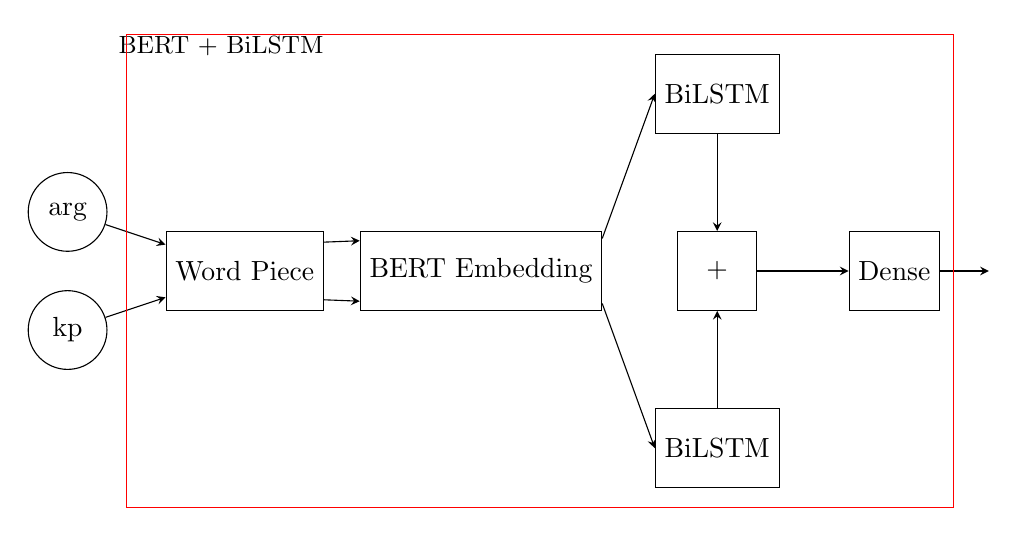
\begin{tikzpicture}[x=1.5cm, y=1.5cm, >=stealth, scale = 1]
      \node [every neuron] (arg) at (0,2.5) {arg};
      \node [every neuron] (kp) at (0,1.5) {kp};
  
      \node [layer] (wp) at (1.5, 2) {Word Piece};
      \node [layer] (be) at (3.5, 2) {BERT Embedding};
  
      \node [layer] (bm1) at (5.5, 3.5) {BiLSTM};
      \node [layer] (bm2) at (5.5, 0.5) {BiLSTM};
  
      \node [layer] (con) at (5.5, 2) {+};
      \node [layer] (den) at (7, 2) {Dense};

      \node [] (des) at (1.3,3.9) {\small BERT + BiLSTM};
  
      \draw [->] (arg) -- (wp);
      \draw [->] (kp) -- (wp);

      \draw [->] (wp.20) -- (be.166);
      \draw [->] (wp.340) -- (be.194);

      \draw [->] (be.15) -- (bm1.180);
      \draw [->] (be.345) -- (bm2.180);

      \draw [->] (bm1.270) -- (con.90);
      \draw [->] (bm2.90) -- (con.270);

      \draw [->] (con) -- (den);

      \draw [->] (den) -- (7.8 ,2);

      \draw[draw=red] (7.5,0) rectangle (0.5,4);
    \end{tikzpicture}
  \end{figure}
\end{frame}

\begin{frame}
  \frametitle{What did work ?}
  \framesubtitle{Combined Model}

  \begin{figure}
    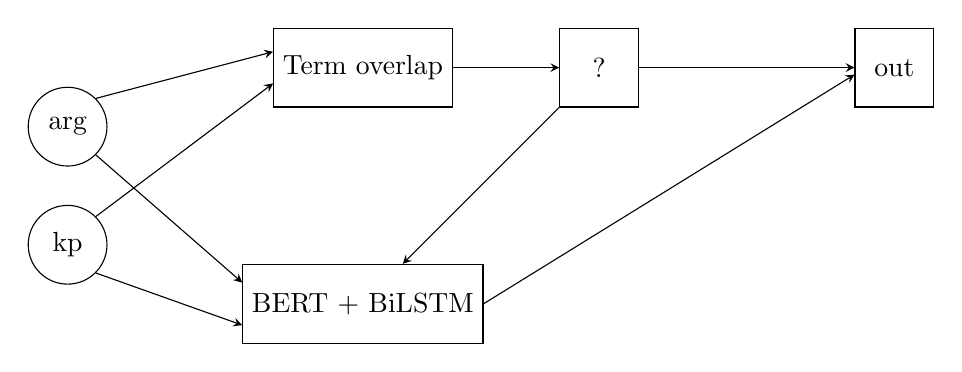
\begin{tikzpicture}[x=1.5cm, y=1.5cm, >=stealth, scale = 1]
      \node [every neuron] (arg) at (0,2.5) {arg};
      \node [every neuron] (kp) at (0,1.5) {kp};
  
      \node [layer] (to) at (2.5, 3) {Term overlap};
      \node [layer] (bb) at (2.5, 1) {BERT + BiLSTM};
  
      \node [layer] (thr) at (4.5, 3) {?};
  
      \node [layer] (out) at (7, 3) {out};

      \draw [->] (arg.45) -- (to.170);
      \draw [->] (kp.45) -- (to.190);

      
      \draw [->] (arg.315) -- (bb.170);
      \draw [->] (kp.315) -- (bb.190);

      \draw [->] (to) -- (thr);
      \draw [->] (thr) -- (bb);
      \draw [->] (thr.0) -- (out);
      \draw [->] (bb.0) -- (out.190);


    \end{tikzpicture}
  \end{figure}
\end{frame}

\begin{frame}
  \frametitle{What does that mean in Scores ?}

  \begin{figure}
    \centering
    \scalebox{.75}{
      \begin{tabular}{lll}
        \toprule
        \multicolumn{1}{c}{\textbf{Approach}} & \multicolumn{1}{c}{\textbf{mAP (str)}} & \multicolumn{1}{c}{\textbf{mAP (rel)}}\\
        \midrule
        term overlap (no preprocessing) &	0.52 & 0.70 \\
        term overlap (stemming) &	0.60 & 0.75\\
        term overlap (stemming, stop words) & 0.64 & 0.81\\
        \textbf{term overlap (stemming, stop words, synonyms, antonyms)}	&	\textbf{0.64}	& \textbf{0.82}\\
        regression (C=1, TF/IDF) & 0.32 & 0.55\\
        regression (C=14, BOW) & 0.44 & 0.70\\
        regression (C=14, BOW, POS) & 0.47 & 0.66\\
        SVC (BOW) & 0.46 & 0.70\\
        SVC (BOW, POS) & 0.48 & 0.74\\
        ensemble (LG=0.55, SVC=0.45, BOW) & 0.43 & 0.64\\
        ensemble (LG=0.55, SVC=0.45, BOW, POS) & 0.50 & 0.70\\
        ensemble (LG=0.45, SVC=0.55, BOW) & 0.45 & 0.65\\
        ensemble (LG=0.45, SVC=0.55, BOW, POS) & 0.51 & 0.71\\
        BiLSTM (GloVe embeddings) & 0.27 & 0.50\\
        \bottomrule
      \end{tabular}
    }
  \end{figure}
\end{frame}

\begin{frame}
  \frametitle{Things to do until the deadline}

  

\end{frame}

\appendix
\section{\appendixname}

\bibliographyframe

\end{document}
